

\tikzset{every picture/.style={line width=0.75pt}} %set default line width to 0.75pt        

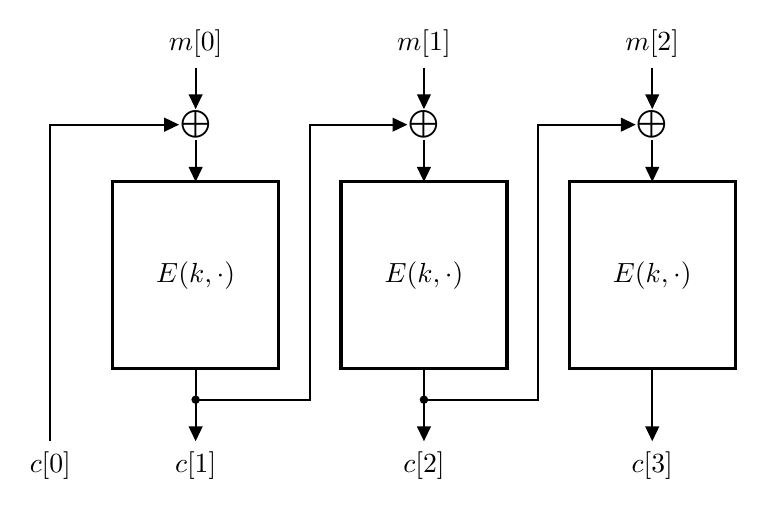
\begin{tikzpicture}[x=0.75pt,y=0.75pt,yscale=-1,xscale=1]
%uncomment if require: \path (0,231); %set diagram left start at 0, and has height of 231

%Shape: Rectangle [id:dp4194833958821309] 
\draw  [line width=1.2]  (45,75) -- (125,75) -- (125,165) -- (45,165) -- cycle ;
%Straight Lines [id:da9137677247487592] 
\draw    (305,165) -- (305,197) ;
\draw [shift={(305,200)}, rotate = 270] [fill={rgb, 255:red, 0; green, 0; blue, 0 }  ][line width=0.08]  [draw opacity=0] (7.14,-3.43) -- (0,0) -- (7.14,3.43) -- cycle    ;
%Straight Lines [id:da6114179035836194] 
\draw    (85,20) -- (85,37) ;
\draw [shift={(85,40)}, rotate = 270] [fill={rgb, 255:red, 0; green, 0; blue, 0 }  ][line width=0.08]  [draw opacity=0] (7.14,-3.43) -- (0,0) -- (7.14,3.43) -- cycle    ;
%Shape: Rectangle [id:dp6391587066292563] 
\draw  [line width=1.2]  (155,75) -- (235,75) -- (235,165) -- (155,165) -- cycle ;
%Straight Lines [id:da22278523727878663] 
\draw    (195,165) -- (195,197) ;
\draw [shift={(195,200)}, rotate = 270] [fill={rgb, 255:red, 0; green, 0; blue, 0 }  ][line width=0.08]  [draw opacity=0] (7.14,-3.43) -- (0,0) -- (7.14,3.43) -- cycle    ;
%Shape: Rectangle [id:dp5279554267177164] 
\draw  [line width=1.2]  (265,75) -- (345,75) -- (345,165) -- (265,165) -- cycle ;
%Straight Lines [id:da9872908902455428] 
\draw    (85,165) -- (85,197) ;
\draw [shift={(85,200)}, rotate = 270] [fill={rgb, 255:red, 0; green, 0; blue, 0 }  ][line width=0.08]  [draw opacity=0] (7.14,-3.43) -- (0,0) -- (7.14,3.43) -- cycle    ;
%Straight Lines [id:da6488866645565632] 
\draw    (85,55) -- (85,72) ;
\draw [shift={(85,75)}, rotate = 270] [fill={rgb, 255:red, 0; green, 0; blue, 0 }  ][line width=0.08]  [draw opacity=0] (7.14,-3.43) -- (0,0) -- (7.14,3.43) -- cycle    ;
%Straight Lines [id:da9196071260539975] 
\draw    (195,20) -- (195,37) ;
\draw [shift={(195,40)}, rotate = 270] [fill={rgb, 255:red, 0; green, 0; blue, 0 }  ][line width=0.08]  [draw opacity=0] (7.14,-3.43) -- (0,0) -- (7.14,3.43) -- cycle    ;
%Straight Lines [id:da34163583536318076] 
\draw    (195,55) -- (195,72) ;
\draw [shift={(195,75)}, rotate = 270] [fill={rgb, 255:red, 0; green, 0; blue, 0 }  ][line width=0.08]  [draw opacity=0] (7.14,-3.43) -- (0,0) -- (7.14,3.43) -- cycle    ;
%Straight Lines [id:da20215887570313607] 
\draw    (305,20) -- (305,37) ;
\draw [shift={(305,40)}, rotate = 270] [fill={rgb, 255:red, 0; green, 0; blue, 0 }  ][line width=0.08]  [draw opacity=0] (7.14,-3.43) -- (0,0) -- (7.14,3.43) -- cycle    ;
%Straight Lines [id:da5146921758845528] 
\draw    (305,55) -- (305,72) ;
\draw [shift={(305,75)}, rotate = 270] [fill={rgb, 255:red, 0; green, 0; blue, 0 }  ][line width=0.08]  [draw opacity=0] (7.14,-3.43) -- (0,0) -- (7.14,3.43) -- cycle    ;
%Straight Lines [id:da3363380063033976] 
\draw    (74,47.5) -- (15,47.5) -- (15,200) ;
\draw [shift={(77,47.5)}, rotate = 180] [fill={rgb, 255:red, 0; green, 0; blue, 0 }  ][line width=0.08]  [draw opacity=0] (7.14,-3.43) -- (0,0) -- (7.14,3.43) -- cycle    ;
%Straight Lines [id:da3504904252774961] 
\draw    (184,47.5) -- (140,47.5) -- (140,180) -- (85,180) ;
\draw [shift={(187,47.5)}, rotate = 180] [fill={rgb, 255:red, 0; green, 0; blue, 0 }  ][line width=0.08]  [draw opacity=0] (7.14,-3.43) -- (0,0) -- (7.14,3.43) -- cycle    ;
%Straight Lines [id:da06499515102720621] 
\draw    (294,47.5) -- (250,47.5) -- (250,180) -- (195,180) ;
\draw [shift={(297,47.5)}, rotate = 180] [fill={rgb, 255:red, 0; green, 0; blue, 0 }  ][line width=0.08]  [draw opacity=0] (7.14,-3.43) -- (0,0) -- (7.14,3.43) -- cycle    ;
%Shape: Circle [id:dp42163039019492987] 
\draw  [fill={rgb, 255:red, 0; green, 0; blue, 0 }  ,fill opacity=1 ] (83.5,180) .. controls (83.5,179.17) and (84.17,178.5) .. (85,178.5) .. controls (85.83,178.5) and (86.5,179.17) .. (86.5,180) .. controls (86.5,180.83) and (85.83,181.5) .. (85,181.5) .. controls (84.17,181.5) and (83.5,180.83) .. (83.5,180) -- cycle ;
%Shape: Circle [id:dp4558022344339028] 
\draw  [fill={rgb, 255:red, 0; green, 0; blue, 0 }  ,fill opacity=1 ] (193.5,180) .. controls (193.5,179.17) and (194.17,178.5) .. (195,178.5) .. controls (195.83,178.5) and (196.5,179.17) .. (196.5,180) .. controls (196.5,180.83) and (195.83,181.5) .. (195,181.5) .. controls (194.17,181.5) and (193.5,180.83) .. (193.5,180) -- cycle ;

% Text Node
\draw (85,120) node    {$E( k,\cdot )$};
% Text Node
\draw (85,16.6) node [anchor=south] [inner sep=0.75pt]    {$m[ 0]$};
% Text Node
\draw (15,203.4) node [anchor=north] [inner sep=0.75pt]    {$c[ 0]$};
% Text Node
\draw (195,120) node    {$E( k,\cdot )$};
% Text Node
\draw (195,16.6) node [anchor=south] [inner sep=0.75pt]    {$m[ 1]$};
% Text Node
\draw (85,203.4) node [anchor=north] [inner sep=0.75pt]    {$c[ 1]$};
% Text Node
\draw (305,120) node    {$E( k,\cdot )$};
% Text Node
\draw (305,16.6) node [anchor=south] [inner sep=0.75pt]    {$m[ 2]$};
% Text Node
\draw (195,203.4) node [anchor=north] [inner sep=0.75pt]    {$c[ 2]$};
% Text Node
\draw (85,47.5) node    {$\bigoplus $};
% Text Node
\draw (195,47.5) node    {$\bigoplus $};
% Text Node
\draw (305,47.5) node    {$\bigoplus $};
% Text Node
\draw (305,203.4) node [anchor=north] [inner sep=0.75pt]    {$c[ 3]$};


\end{tikzpicture}